%!TEX root = <main.tex>
\section{Experimental Evaluation}
We empirically validate if \system~ is able reduce the runtime take for occlusion based deep CNN explainability workloads.
We then conduct conduct controlled experiments to show the individual contribution of each optimization in \system~ for the overall system speedup.

\subsection{End-to-End Evaluation}

\vspace{2mm}
\noindent \textbf{Datasets.}

\vspace{2mm}
\noindent \textbf{Workloads.}

\vspace{2mm}
\noindent \textbf{Experimental Setup.}

\subsection{Lesion Study}

\vspace{2mm}
\noindent \textbf{Speedups from Incremental Inference.}
\begin{figure}[t]
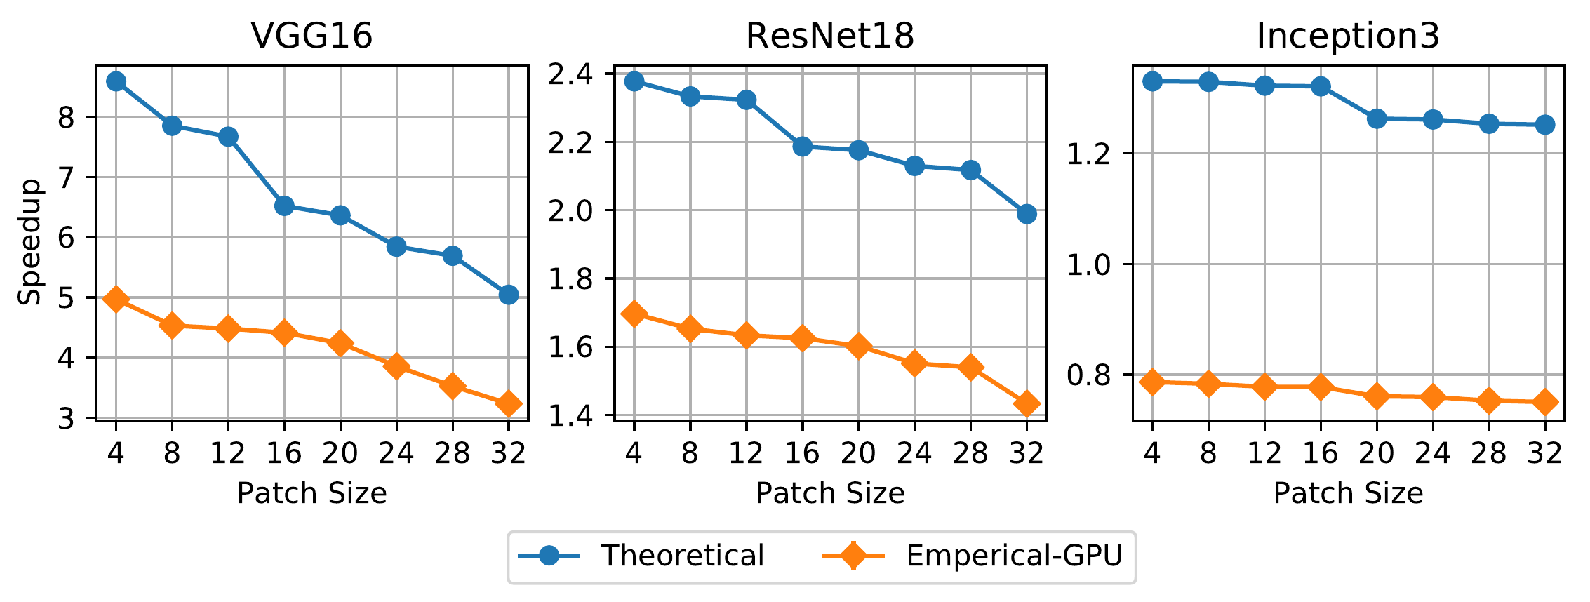
\includegraphics[width=\columnwidth]{images/5_2_1_GPU}
\caption{Theoretical versus empirical speedup for \textit{incremental inference} with varying occlusion patch sizes and different CNN models (Occlusion patch stride $S=1$).}
\label{fig:5_2_1_GPU}
\end{figure}

\vspace{2mm}
\noindent \textbf{Speedups from Projective Field Thresholding.}
\begin{figure}[t]
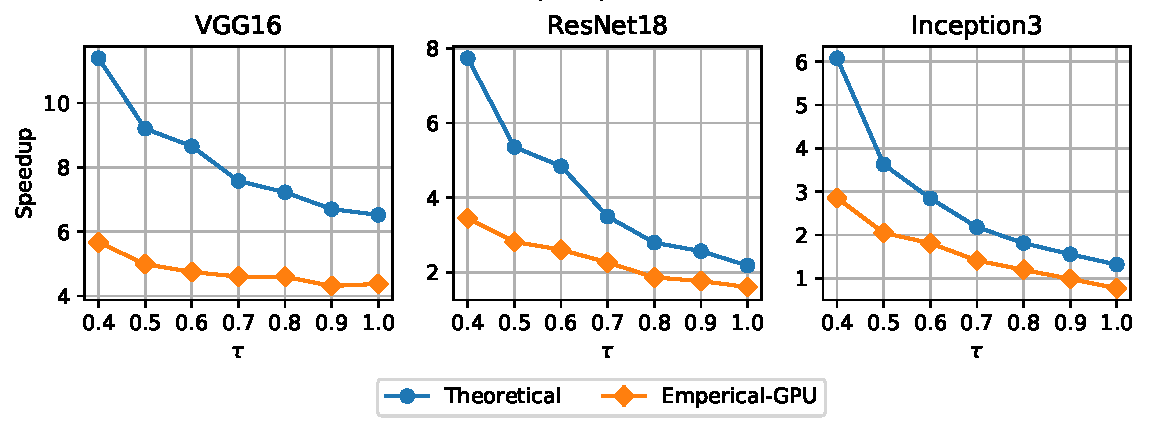
\includegraphics[width=\columnwidth]{images/5_2_2_GPU}
\caption{Theoretical versus empirical speedup for \textit{incremental inference} with \textit{projective field thresholding} with varying threshold values ($\tau$) and different CNN models (Occlusion patch size = $16 \times 16$, stride $S=1$).}
\label{fig:5_2_1_GPU}
\end{figure}

\vspace{2mm}
\noindent \textbf{Speedups from Adaptive Drill-Down.}

\begin{figure}[t]
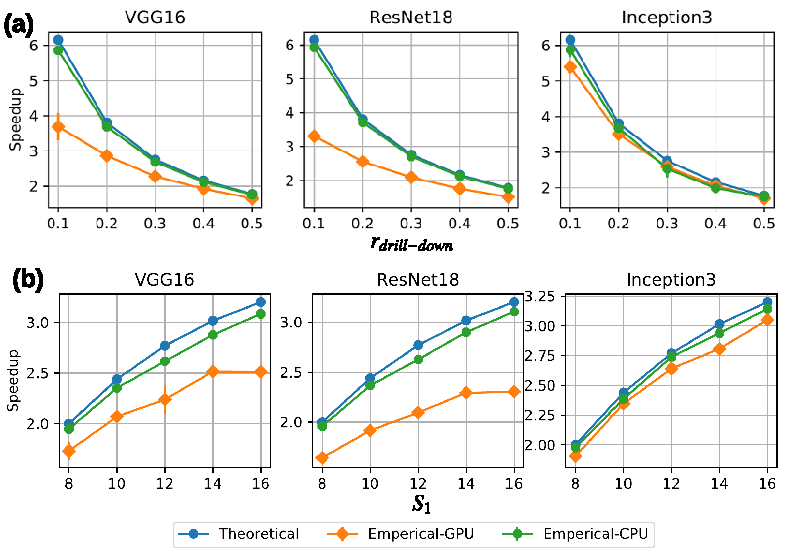
\includegraphics[width=\columnwidth]{images/5_2_3_GPU}
\caption{Theoretical versus empirical speedup for \textit{adaptive drill-down} with (a) varying drill-down ratios ($r_{drill-down}$) and (b) varying stage one stride $S_1$ values for different CNN models (Occlusion patch size = $16 \times 16$, stage two stride $S_2=1$, projective field threshold $\tau=1.0$).}
\label{fig:5_2_3_GPU}
\end{figure}

\vspace{2mm}
\noindent \textbf{Summary of Experimental Results.}

\subsection{Discussion and Limitations}